% Options for packages loaded elsewhere
\PassOptionsToPackage{unicode}{hyperref}
\PassOptionsToPackage{hyphens}{url}
\PassOptionsToPackage{dvipsnames,svgnames,x11names}{xcolor}
%
\documentclass[
  number]{elsarticle}

\usepackage{amsmath,amssymb}
\usepackage{iftex}
\ifPDFTeX
  \usepackage[T1]{fontenc}
  \usepackage[utf8]{inputenc}
  \usepackage{textcomp} % provide euro and other symbols
\else % if luatex or xetex
  \usepackage{unicode-math}
  \defaultfontfeatures{Scale=MatchLowercase}
  \defaultfontfeatures[\rmfamily]{Ligatures=TeX,Scale=1}
\fi
\usepackage{lmodern}
\ifPDFTeX\else  
    % xetex/luatex font selection
  \setmainfont[]{Times New Roman}
  \setmonofont[]{DejaVu Sans Mono}
\fi
% Use upquote if available, for straight quotes in verbatim environments
\IfFileExists{upquote.sty}{\usepackage{upquote}}{}
\IfFileExists{microtype.sty}{% use microtype if available
  \usepackage[]{microtype}
  \UseMicrotypeSet[protrusion]{basicmath} % disable protrusion for tt fonts
}{}
\makeatletter
\@ifundefined{KOMAClassName}{% if non-KOMA class
  \IfFileExists{parskip.sty}{%
    \usepackage{parskip}
  }{% else
    \setlength{\parindent}{0pt}
    \setlength{\parskip}{6pt plus 2pt minus 1pt}}
}{% if KOMA class
  \KOMAoptions{parskip=half}}
\makeatother
\usepackage{xcolor}
\setlength{\emergencystretch}{3em} % prevent overfull lines
\setcounter{secnumdepth}{-\maxdimen} % remove section numbering
% Make \paragraph and \subparagraph free-standing
\ifx\paragraph\undefined\else
  \let\oldparagraph\paragraph
  \renewcommand{\paragraph}[1]{\oldparagraph{#1}\mbox{}}
\fi
\ifx\subparagraph\undefined\else
  \let\oldsubparagraph\subparagraph
  \renewcommand{\subparagraph}[1]{\oldsubparagraph{#1}\mbox{}}
\fi


\providecommand{\tightlist}{%
  \setlength{\itemsep}{0pt}\setlength{\parskip}{0pt}}\usepackage{longtable,booktabs,array}
\usepackage{calc} % for calculating minipage widths
% Correct order of tables after \paragraph or \subparagraph
\usepackage{etoolbox}
\makeatletter
\patchcmd\longtable{\par}{\if@noskipsec\mbox{}\fi\par}{}{}
\makeatother
% Allow footnotes in longtable head/foot
\IfFileExists{footnotehyper.sty}{\usepackage{footnotehyper}}{\usepackage{footnote}}
\makesavenoteenv{longtable}
\usepackage{graphicx}
\makeatletter
\def\maxwidth{\ifdim\Gin@nat@width>\linewidth\linewidth\else\Gin@nat@width\fi}
\def\maxheight{\ifdim\Gin@nat@height>\textheight\textheight\else\Gin@nat@height\fi}
\makeatother
% Scale images if necessary, so that they will not overflow the page
% margins by default, and it is still possible to overwrite the defaults
% using explicit options in \includegraphics[width, height, ...]{}
\setkeys{Gin}{width=\maxwidth,height=\maxheight,keepaspectratio}
% Set default figure placement to htbp
\makeatletter
\def\fps@figure{htbp}
\makeatother

\usepackage{booktabs}
\usepackage{caption}
\usepackage{longtable}
\makeatletter
\makeatother
\makeatletter
\makeatother
\makeatletter
\@ifpackageloaded{caption}{}{\usepackage{caption}}
\AtBeginDocument{%
\ifdefined\contentsname
  \renewcommand*\contentsname{Table of contents}
\else
  \newcommand\contentsname{Table of contents}
\fi
\ifdefined\listfigurename
  \renewcommand*\listfigurename{List of Figures}
\else
  \newcommand\listfigurename{List of Figures}
\fi
\ifdefined\listtablename
  \renewcommand*\listtablename{List of Tables}
\else
  \newcommand\listtablename{List of Tables}
\fi
\ifdefined\figurename
  \renewcommand*\figurename{Figure}
\else
  \newcommand\figurename{Figure}
\fi
\ifdefined\tablename
  \renewcommand*\tablename{Table}
\else
  \newcommand\tablename{Table}
\fi
}
\@ifpackageloaded{float}{}{\usepackage{float}}
\floatstyle{ruled}
\@ifundefined{c@chapter}{\newfloat{codelisting}{h}{lop}}{\newfloat{codelisting}{h}{lop}[chapter]}
\floatname{codelisting}{Listing}
\newcommand*\listoflistings{\listof{codelisting}{List of Listings}}
\makeatother
\makeatletter
\@ifpackageloaded{caption}{}{\usepackage{caption}}
\@ifpackageloaded{subcaption}{}{\usepackage{subcaption}}
\makeatother
\makeatletter
\@ifpackageloaded{tcolorbox}{}{\usepackage[skins,breakable]{tcolorbox}}
\makeatother
\makeatletter
\@ifundefined{shadecolor}{\definecolor{shadecolor}{rgb}{.97, .97, .97}}
\makeatother
\makeatletter
\makeatother
\makeatletter
\makeatother
\ifLuaTeX
  \usepackage{selnolig}  % disable illegal ligatures
\fi
\usepackage[]{natbib}
\bibliographystyle{elsarticle-num}
\IfFileExists{bookmark.sty}{\usepackage{bookmark}}{\usepackage{hyperref}}
\IfFileExists{xurl.sty}{\usepackage{xurl}}{} % add URL line breaks if available
\urlstyle{same} % disable monospaced font for URLs
\hypersetup{
  pdftitle={HEPA Air Filters for Preventing Wildfire-Related Asthma Complications, a Cost-effectiveness Study},
  pdfauthor={Amin Adibi; Prabjit Barn; Erin M Shellington; Stephanie Harvard; Kate Johnson (* co-senior author); Christopher Carlsten (* co-senior author)},
  colorlinks=true,
  linkcolor={blue},
  filecolor={Maroon},
  citecolor={Blue},
  urlcolor={Blue},
  pdfcreator={LaTeX via pandoc}}

\setlength{\parindent}{6pt}
\begin{document}

\begin{frontmatter}
\title{HEPA Air Filters for Preventing Wildfire-Related Asthma
Complications, a Cost-effectiveness Study}
\author[1,2]{Amin Adibi%
%
}
 \ead{amin.adibi@ubc.ca} 
\author[3]{Prabjit Barn%
%
}

\author[4,5]{Erin M Shellington%
%
}

\author[2]{Stephanie Harvard%
%
}

\author[1,4,5,2]{Kate Johnson (* co-senior author)%
%
}

\author[4,5,6]{Christopher Carlsten (* co-senior author)%
\corref{cor1}%
}


\affiliation[1]{organization={Climate Change Health Effects, Adaptation,
and ResiLience (HEAL) Research Cluster, University of British
Columbia},,postcodesep={}}
\affiliation[2]{organization={Respiratory Evaluation Sciences Program,
Collaboration for Outcomes Research and Evaluation, Faculty of
Pharmaceutical Sciences, University of British
Columbia},,postcodesep={}}
\affiliation[3]{organization={Fraser Health Authority},,postcodesep={}}
\affiliation[4]{organization={Legacy for Airway Health, Vancouver
Coastal Health Research Institute},,postcodesep={}}
\affiliation[5]{organization={Division of Respiratory Medicine, Faculty
of Medicine, University of British Columbia},,postcodesep={}}
\affiliation[6]{organization={Air Pollution Exposure Lab, Vancouver
Coastal Health Research Institute},,postcodesep={}}

\cortext[cor1]{Corresponding author}






        
\begin{abstract}
\textbf{RATIONALE:} The number, size, and intensity of wildfires have
increased in Canada, particularly in the western province of British
Columbia (BC). Air pollution caused by wildfire smoke is linked to
adverse health outcomes, especially for people living with asthma.
Portable high-efficiency particulate air (HEPA) filters are effective at
reducing indoor air concentrations of particulate matter associated with
wildfire smoke. Using historical concentrations of particulate matter
from wildfire smoke, we evaluated the cost-effectiveness of a
government-sponsored HEPA air filter rebate program to improve asthma
control and prevent exacerbations across Health Service Delivery Areas
(HSDAs) in BC, Canada.

\textbf{METHODS:} We developed a time-varying Markov model with health
states for levels of asthma control, exacerbation severity (defined
based on medication use, emergency department visits, and
hospitalizations), and death. The analysis was performed from the
healthcare payer perspective over a retrospective time horizon of 5
years (2018-2022). We obtained average daily concentrations of wildfire
smoke-derived particulate matter of less than or equal to 2.5 microns in
diameter (PM\textsubscript{2.5}) for each HSDA from the Canadian
Optimized Statistical Smoke Model. Clinical inputs were informed by the
literature. We ran the model for the base case (full rebate and
continuous year-round operation of air filters) and scenarios (variable
rebate of \$100 {[}67\% of purchase cost{]} and \$30 {[}20\% of purchase
cost{]} and either continuous or threshold-based operation of air
filters) in each HSDA in BC and calculated quality-adjusted life-years
(QALYs) and costs. Incremental cost-effectiveness ratios (ICERs) were
compared to a willingness-to-pay (WTP) threshold of \$50,000/QALY.

\textbf{RESULTS:} In the base case analysis, HEPA air filter use
resulted in increased costs of \$82.84 (SE=1.05) and increased QALYs of
0.0012 (SE=0.0001) per person. Average ICER among BC HSDAs was
\$71,477/QALY (SE=3,378), with ICERs ranging from \$38,628 to \$85,445
per QALY in HSDAs. Across the province, the intervention was projected
to prevent 4,536 exacerbations requiring systemic corticosteroids, 531
emergency department visits, and 458 hospitalizations during the 5-year
time horizon. A full rebate was cost-effective in one of the 16 HSDAs
across BC. The probability of cost-effectiveness ranged from 0.3\% to
80.2\% across HSDAs. A \$100 rebate was cost-effective in all HSDAs
except Northwest.

\textbf{CONCLUSIONS:} Our retrospective modelling suggests variable
cost-effectiveness of portable HEPA air filters to reduce short-term
asthma complications due to wildfire smoke, dependent on region and
percentage of government rebate on the purchase cost of these filters.
At the willingness-to-pay threshold of \$50,000/QALY, rebates of up to
two-thirds of the cost of filters were a cost-effective alternative
across most of the geography of the province. However, it would be
cost-effective for the BC government to provide a 100\% rebate only in
Kootenay Boundary.
\end{abstract}





\end{frontmatter}
    \ifdefined\Shaded\renewenvironment{Shaded}{\begin{tcolorbox}[breakable, enhanced, sharp corners, interior hidden, boxrule=0pt, frame hidden, borderline west={3pt}{0pt}{shadecolor}]}{\end{tcolorbox}}\fi

\hypertarget{lay-summary}{%
\subsection{Lay Summary}\label{lay-summary}}

Wildfire smoke can increase flare up of symptoms among people living
with asthma. These flare ups may require a visit to the emergency
department or hospital admission. Research shows that portable HEPA air
filters can significantly reduce concentrations of fine particles
(PM\textsubscript{2.5}, an important component of wildfire smoke) in
homes and other buildings. Using air filters during smoke events is a
common public health recommendation. However, air filters are not
accessible to everyone, with units costing anywhere between \$150 to a
few hundred dollars. Does it make sense for the government of BC to
offer a rebate on the cost of purchasing air filters for every person
living with asthma in BC? In this study, we used historical data on
wildfire smoke concentrations between 2018 to 2022, computer
simulations, and health economics methods to answer this question. Our
results suggest that it is likely cost-effective for the government to
pay for a portion of the costs of air filters, particularly in the
interior and northern interior parts of BC. We also looked at other
scenarios, such as filter use only when outdoor pollution exceeds
certain thresholds that typically trigger an air quality advisory. We
found that a \$100 rebate was cost-effective when the air filter was
used continuously, whereas a \$30 rebate was cost-effective when the air
filter was turned on only during air quality advisories.

\hypertarget{background}{%
\section{Background}\label{background}}

The number, size, and intensity of wildfires in Canada have increased,
particularly in the western province of British Columbia (BC) with the
number of days with uncontrolled wildfire in BC expected to double or
triple by 2100\citep{wotton2017}.

Wildfire smoke is composed of several pollutants, including fine
particulate matter with diameters of 2.5 microns and smaller
(PM\textsubscript{2.5}). PM\textsubscript{2.5} and other air pollutants
have been associated with increased respiratory symptoms,
hospitalizations, and other adverse health effects in individuals with
asthma \citep{reid2016}.

People living with asthma are particularly susceptible to air pollution.
Asthma exacerbations (also known as \emph{flare-ups} or \emph{acute
severe asthma}) are episodes characterized by progressive worsening of
cough, wheezing, shortness of breath and decrease in lung function
\citep{globalinitiativeforasthma2022}. Severe exacerbations can be fatal
and can occur even in patients with well-controlled asthma
\citep{globalinitiativeforasthma2022}. Previous studies have shown that
PM\textsubscript{2.5} from wildfire events can increase the risk of
asthma exacerbations \citep{borchers_arriagada_association_2019}.

During wildfire smoke events, indoor PM\textsubscript{2.5}
concentrations increase as smoke infiltrates into homes and other
buildings. Because people typically spend \textgreater70\% of their time
in indoor environments, \citep{statisticscanadageneralsocialsurvey}
indoor air quality is an important contributor to total air pollution
exposure. Consequently, interventions that improve indoor air quality
are important to protecting health, particularly during episodes of poor
air quality, such as during wildfire smoke events. Portable
high-efficiency particulate air (HEPA) filters can reduce indoor
concentrations of PM\textsubscript{2.5}\citep{zhu2021}. These units work
by drawing air across a highly efficient filter that traps particles,
including PM\textsubscript{2.5}, and release filtered air. HEPA and
other filters can be portable, or be part of a buildings heating,
ventilation, and air conditioning (HVAC) system, and often referred to
induct filters.

As the climate emergency worsens and continues to impact air
quality\citep{kirchmeier-young2019}, there is growing consensus among
the public health community that using air filters in indoor settings is
an important health-protective intervention, particularly for vulnerable
people. The Government of Canada currently provides tax benefits for the
full cost of an air filter, cleaner, or purifier and up to \$1000 for
the purchase of an air conditioner for patients living with a chronic
disease who have a prescription for these devices
\citep{canadarevenueagency2016}. In 2021, the Canadian Government also
announced a 25\% tax credit for small businesses to upgrade their
ventilation systems and purchase portable HEPA air filters
\citep{departmentoffinancegovernmentofcanada2021}. In BC, the First
Nations Health Authority (FNHA) provides portable air filters to
communities affected by wildfires
\citep{firstnationshealthauthority2022}. We are also aware of two
similar programs in the US: an air filter distribution program for
low-income asthma patients by the Bay Area Air Quality and Management
District \citep{thebayareaairqualityandmanagementdistrict2021}, and a
HEPA filter loaner program by the Forest Stewards Guild in Santa Fe
\citep{participant2020}. However, we are not aware of any formal
analysis evaluating the cost-effectiveness of these programs from a
health economics perspective.

In this study, we used a decision-analytic model to evaluate the
cost-effectiveness of a government-sponsored portable HEPA air filters
rebate program for improving asthma control and preventing asthma
exacerbations caused by wildfire events in BC, Canada. Our analysis can
serve as a blueprint for evaluating similar climate change adaptation
strategies in BC and elsewhere.

\hypertarget{methods}{%
\section{Methods}\label{methods}}

We have reported the results of this study according to the
recommendations and best practices set forth in the Consolidated Health
Economic Evaluation Reporting Standards 2022 (CHEERS 2022) statement
\citep{husereau2022}.

Our base case analysis assumes that the provincial government will offer
a 100\% rebate for portable HEPA air filters to all individuals
diagnosed with asthma in BC. We used a retrospective time horizon of
five years beginning in 2018 to the end of 2022, which was the most
recent 5-year time horizon for which the data were available. This
retrospective time horizon was necessary as daily projections of future
wildfire PM\textsubscript{2.5} concentrations are not available. We
assumed patients on average spent 69.6\% of their time at home (and thus
could benefit from the air filter for the proportion of time they were
at home), based on the time use information collected in Statistics
Canada's General Social Survey
\citep{statisticscanadageneralsocialsurvey}. The target population was
BC residents diagnosed with asthma with a starting age of 42 (the
average age of BC residents)\citep{governmentofcanada2017}.

We projected costs in 2023 Canadian dollar and effects as
Quality-Adjusted Life Years (QALYs) for patients with and without
portable HEPA air filters in their homes, and report results for each
Health Service Delivery Area (HSDA) in BC. We also report the number of
averted cases of asthma exacerbations using model-projected exacerbation
rates and crude asthma prevalence levels from April 1st, 2020 to March
31st, 2021 for each HSDA obtained from
BCCDC\citep{britishcolumbiaministryofhealth}. We calculated Incremental
Cost-effectiveness Ratios (ICER) and Net-Monetary Benefit (NMB) and
reported cost-effectiveness at willingness-to-pay (WTP) threshold of
\$50,000/QALY.

The analysis was conducted from the healthcare payer perspective, with
an annual discounting of 1.5\% applied to costs and effects.

\hypertarget{stakeholder-engagement}{%
\subsection{Stakeholder engagement}\label{stakeholder-engagement}}

We developed a health economic analysis plan with early and ongoing
input from stakeholders, including two patient partners living with
asthma, two medical health officers, an environment health officer, and
a policy analyst (see Acknowledgment section).

\hypertarget{model-development}{%
\subsection{Model development}\label{model-development}}

We developed a time-varying Markov model with seven health states
corresponding to well-controlled asthma, partly-controlled asthma, and
uncontrolled asthma (as defined per Global Initiative for Asthma (GINA)
2022 \citep{globalinitiativeforasthma2022}) as well as exacerbations
requiring either systemic corticosteroids (ExacSCS), a visit to the
Emergency Department (ExacED), or hospitalization (ExacHosp), and death,
respectively (Figure~\ref{fig-markov}).

Background mortality was based on age-specific life tables for BC from
Statistics Canada \citep{statisticscanada2022}. Mortality due to asthma
exacerbations of each severity was based on a national review of asthma
deaths in the UK \citep{watson2007, levy2014asthma}. Annual transition
probabilities between asthma control states were based on an original
analysis of Economic Burden of Asthma study where we calculated the
proportion of transitions occurring between each control state over 5
visits conducted over 1 year of follow-up \citep{sadatsafavi2015}. Rates
of severe exacerbations leading to SCS, ED, or hospitalization were
obtained from SYGMA II study\citep{bateman2018}. We applied a risk ratio
of 1.40 to individuals with partially controlled and uncontrolled asthma
to reflect their higher probability of exacerbations. This parameter was
based on an analysis of commercially insured patients in the
US\citep{pollack2022}.

We ran the model using daily time cycles.

\begin{figure}

{\centering \includegraphics{markov.png}

}

\caption{\label{fig-markov}Markov health states and transitions}

\end{figure}

\hypertarget{air-pollution-exposure}{%
\subsection{Air Pollution Exposure}\label{air-pollution-exposure}}

Average daily outdoor PM\textsubscript{2.5} concentrations were obtained
from CanOSSEM \citep{PAUL2022157956}, a random forest machine learning
model developed and validated by BC Center for Disease Control that
projects retrospective average daily wildfire smoke levels for each
postal code in BC. Outdoor PM\textsubscript{2.5} concentrations in HSDAs
were obtained by linking postal codes to HSDAs using Postal Code
Conversion File Plus (PCCF+) Version 7E\citep{AB2/D1AO5H_2022}. Model
assumptions are listed in Table~\ref{tbl-assumptions}.

Risk ratios for the effect of increased exposure to
PM\textsubscript{2.5} on asthma outcomes, including salbutamol
dispensation and asthma-related physician visit, ED visit, and
hospitalizations were obtained from a recent
meta-analysis\citep{borchers_arriagada_association_2019} and a model
validation study based on BC administrative health data \citep{yao2014}.

\hypertarget{tbl-assumptions}{}
\begin{longtable}[]{@{}
  >{\raggedright\arraybackslash}p{(\columnwidth - 0\tabcolsep) * \real{1.0039}}@{}}
\caption{\label{tbl-assumptions}Model assumptions for evaluating
cost-effectiveness of a portable air filter rebate program to prevent
asthma exacerbations}\tabularnewline
\toprule\noalign{}
\begin{minipage}[b]{\linewidth}\raggedright
Assumptions for base case analysis
\end{minipage} \\
\midrule\noalign{}
\endfirsthead
\toprule\noalign{}
\begin{minipage}[b]{\linewidth}\raggedright
Assumptions for base case analysis
\end{minipage} \\
\midrule\noalign{}
\endhead
\bottomrule\noalign{}
\endlastfoot
HEPA air filters were assumed to operate continuously on their highest
setting during model's time horizon. \\
We assumed that the government could offer rebates at a discount of 30\%
compared to the advertised retail price. \\
We assumed that HEPA filters will need to be replaced every 9 months of
use based on the average manufacturer-recommended timeline, while the
filtration unit will need to be replaced every five years regardless of
how much it was used. \\
Residents were assumed to cover the cost of electricity and filter
replacement. \\
We assumed that people living with asthma received one HEPA air filter
unit each, even if there were multiple people with asthma in the same
home. We assumed that air filters were placed in the main living space
or main bedroom of the person with asthma. \\
We assumed people living with asthma spent the same proportion of their
day at home as the general population. \\
Increased salbutamol dispensation (per canister) per 10 µg/m³ increase
in PM\textsubscript{2.5} during wildfire events was used as a proxy for
risk of worsened asthma control (ie. well controlled to partly
controlled, or partly controlled to uncontrolled). \\
Potential additional benefits of HEPA air filters in reducing exposure
to allergens, pathogens, and indoor sources of PM\textsubscript{2.5}
such as cooking or wood stoves were not considered. \\
We assumed all patients would enter the ``uncontrolled asthma'' health
state after an exacerbation event. \\
Historical wildfire-related PM\textsubscript{2.5} levels projected by
the CanOSSEM model were assumed to be accurate. \\
\end{longtable}

Transition probabilities, utility and disutility values, rate ratios for
the effect of increased PM\textsubscript{2.5} pollution on asthma
outcomes, healthcare state costs, outdoor to indoor
PM\textsubscript{2.5} infiltration rates, and HEPA filter efficiency
rate were obtained from the literature (Table~\ref{tbl-parameters}).

\hypertarget{hepa-air-filter-effectiveness}{%
\subsection{HEPA Air Filter
Effectiveness}\label{hepa-air-filter-effectiveness}}

We chose what we considered to be a \emph{typical} HEPA air filter unit
with a clean air delivery rate (CADR) of 105 cfm for smoke, and a
nominal air exchange rate of 4.8/hr for a coverage area of 15
m\textsuperscript{2}. Measured HEPA filter efficiency of 0.31 (defined
as the ratio of indoor PM\textsubscript{2.5} measured throughout the
year with HEPA to without HEPA filter) was obtained from a study led by
one of our co-authors that evaluated air filter effectiveness in BC
homes during smoke events \citep{Barn2008} using a comparable air filter
unit with a CADR of 150 cfm and nominal air exchange rate of 6/hr for a
coverage area of 17.37 m\textsuperscript{2}
(Table~\ref{tbl-parameters}). Varying filter effectiveness values of
(±20\%) were explored in one-way sensitivity analysis.

\hypertarget{costs}{%
\subsection{Costs}\label{costs}}

Costs included the initial purchase price of the HEPA air filter unit,
background healthcare costs based on asthma control level, and unit
costs of exacerbations obtained from the literature. Unit costs and
utilization were obtained from previous
studies\citep{sadatsafavi2021, bateman2018}.

Costs to patients for air filter operation such as electricity and
replacement HEPA filters after every 9 months of use (based average
replacement duration according to the manufacturer) were not included in
the base case analysis, but are reported in scenario analysis.

\hypertarget{health-state-utilities}{%
\subsection{Health State Utilities}\label{health-state-utilities}}

Health state utilities were derived from the literature based on levels
of asthma control, while severe exacerbations requiring systemic SCS, ED
visit, or hospitalization were associated with a one-time disutility
value derived from EQ-5D questionnaires \citep{lloyd2007}.

\hypertarget{sensitivity-analyses}{%
\subsection{Sensitivity Analyses}\label{sensitivity-analyses}}

One-way deterministic sensitivity analysis was used to explore the
effect of changing assumptions on the estimated costs and QALYs.
Uncertainty in the results due to parameter uncertainty was explored
through probabilistic sensitivity analysis with 1000 sampling from
parameters distributions (Table~\ref{tbl-parameters}) in each HSDA.

Our base case scenario assumed that the government covered the full cost
of the air filter and that air filters were operating continuously
throughout the five years of study. Here, we explore three different
scenarios: 1) the government pays a \$100 (67\%) rebate, 2) the
government pays a full (100\%) rebate and air filters are turned on only
when the outdoor pollution exceeds certain thresholds, and 3) the
government pays a \$30 (20\%) rebate and the air filter operates only
when outdoor PM\textsubscript{2.5} concentration is above a certain
threshold. We chose rebate amounts based on convenience and existing
provincial rebate programs (e.g.~for energy efficient products
\citep{bchydro}).

\hypertarget{software}{%
\subsection{Software}\label{software}}

Data preparation, model development, and statistical analysis was
performed in R v4.2.3 using the \emph{heemod} package v0.15.1
\citep{filipovic-pierucci2016}. We used Quarto v1.3.326 to create a
reproducible manuscript and used version control to keep track of
methodological decisions and changes to the model.

\hypertarget{tbl-parameters}{}
\begin{longtable}[]{@{}
  >{\raggedright\arraybackslash}p{(\columnwidth - 8\tabcolsep) * \real{0.4824}}
  >{\raggedright\arraybackslash}p{(\columnwidth - 8\tabcolsep) * \real{0.1106}}
  >{\raggedright\arraybackslash}p{(\columnwidth - 8\tabcolsep) * \real{0.0754}}
  >{\raggedright\arraybackslash}p{(\columnwidth - 8\tabcolsep) * \real{0.1005}}
  >{\raggedright\arraybackslash}p{(\columnwidth - 8\tabcolsep) * \real{0.2161}}@{}}
\caption{\label{tbl-parameters}Model Parameters}\tabularnewline
\toprule\noalign{}
\endfirsthead
\endhead
\bottomrule\noalign{}
\endlastfoot
\textbf{Parameter} & \textbf{Base case} & \textbf{DSA} & \textbf{PSA} &
\textbf{Source} \\
Age at start & 42 & 33\textbar67 & & \citep{governmentofcanada2017} \\
Mean infiltration efficiency without HEPA & 61\% & & Normal (SD=0.27) &
\citep{Barn2008} \\
Mean infiltration efficiency with HEPA & 19\% & & Normal (SD=0.20) &
\citep{Barn2008} \\
Filter Effect & 31\% & ±20\% & Beta & \citep{Barn2008, zhu2021} \\
RR for increased salbutamol dispensation per 10 µg/m³ increase in
PM\textsubscript{2.5} & 1.04 {[}1.03-1.06{]} & 1\textbar1.20 & Lognormal
& \citep{yao2014} \\
RR for increased physician visit for asthma per 10 µg/m³ increase in
PM\textsubscript{2.5} & 1.06 {[}1.04--1.08{]} & 1\textbar1.20 &
Lognormal & \citep{yao2014} \\
RR for asthma related ED visit per 10 µg/m³ increase in
PM\textsubscript{2.5} & 1.07 {[}1.04--1.09{]} & 1\textbar1.20 &
Lognormal & \citep{borchers_arriagada_association_2019} \\
RR for asthma related hospitalization per 10 µg/m³ increase in
PM\textsubscript{2.5} & 1.06 (1.02--1.09) & 1\textbar1.20 & Lognormal &
\citep{borchers_arriagada_association_2019} \\
Probabilities\footnote{Annual and monthly probabilities were converted
  rescaled to daily probabilities using \(p_m=1-(1-p)^{(1/n)}\)} & & &
& \\
Risk of death due to exacerbation (SCS) & 0.0267\% & & Beta &
\citep{watson2007, levy2014asthma} \\
Risk of death due to exacerbation (ED) & 0.1733\% & & Beta &
\citep{watson2007, levy2014asthma} \\
Risk of death due to exacerbation (hospitalization) & 0.1801\% & & Beta
& \citep{watson2007, roberts2013} \\
Well-controlled to uncontrolled asthma, annually & 14.52\% & & Beta &
\citep{sadatsafavi2015} \\
Well-controlled to partly-controlled, annually & 81.28\% & & Beta &
\citep{sadatsafavi2015} \\
Partly-controlled to well-controlled, annually & 72.03\% & & Beta &
\citep{sadatsafavi2015} \\
Partly-controlled to uncontrolled, annually & 67.94\% & & Beta &
\citep{sadatsafavi2015} \\
Uncontrolled to partly controlled, annually & 79.21\% & & Beta &
\citep{sadatsafavi2015} \\
Uncontrolled to well-controlled asthma, annually & 38.34\% & & Beta &
\citep{sadatsafavi2015} \\
Annual rate of exacerbation (SCS) in controlled asthma & 0.0845

p=8.05\%\footnote{Per Table 1 in Bateman et al. \citep{bateman2018},
  45.9\% of patients had uncontrolled asthma, while 54.1\% had
  controlled asthma. Per \citep{bateman2018} the overall annual rate of
  exacerbations (SCS) was 0.1, which translates to an annual probability
  of 0.09516. We combined this information with risk ratios for asthma
  control level and exacerbations from \citep{pollack2022} to solve for
  the annual exacerbation risks for those with controlled asthma:

  \(0.541 \times x+0.459 \times x \times1.397727 = 0.09516\) so
  \(x \approx 0.08047\)} & & Beta & \citep{bateman2018, pollack2022} \\
Annual rate of exacerbation (ED) in controlled asthma & 0.0084

p=0.84\% & & Beta & \citep{bateman2018, pollack2022} \\
Annual rate of exacerbation (hospitalization) in controlled asthma &
0.0084

p=0.84\% & & Beta & \citep{bateman2018, pollack2022} \\
RR for exacerbations (SCS, ED, or hospitalization) in uncontrolled
asthma vs.~well-controlled & 1.3977 & ±20\% & Lognormal &
\citep{pollack2022} \\
RR for exacerbations in partly controlled asthma vs.~well-controlled &
0.9545 & ±20\% & Lognormal & \citep{pollack2022} \\
Exacerbation (SCS, ED, or hospitalization) to uncontrolled asthma &
1-p\_mortality & & Fixed & \\
& & & & \\
\textbf{Exposures} & & & & \\
Monthly PM\textsubscript{2.5} levels (either as average for each postal
code & \begin{minipage}[t]{\linewidth}\raggedright
\hfill\break
CanOSSEM\strut
\end{minipage} & & Fixed & \citep{PAUL2022157956} \\
& & & & \\
\textbf{Unit Costs} & & & & \\
HEPA air filter unit & \$150 & ±20\% & Gamma & Retail Price \\
government discount on retail price & 30\% & & Assumption & \\
Indoor HEPA air filter electricity usage, annually (when used
continuously) & \begin{minipage}[t]{\linewidth}\raggedright
\$9.90\\
\strut
\end{minipage} & Fixed & Fixed & BC Hydro Calculator \footnote{Calculations
  are based on Blue Pure 411 Auto running at highest setting (10W) for
  24 hours every day for a year (87.60 kWh) at an average residential
  rate of 11.30 cents per kWh (a blend of step 1 and step 2 rates). For
  more info, see
  https://www.bchydro.com/powersmart/residential/tools-and-calculators/cost-calculator.html} \\
Filter Replacement, per replacement &
\begin{minipage}[t]{\linewidth}\raggedright
\$30\\
\strut
\end{minipage} & ±20\% & Gamma & Retail Price \\
Direct costs of well-controlled asthma, monthly & \$323.57 & ±20\% &
Normal (SD=59.50) & \citep{yaghoubi2020} \\
Direct costs of partly controlled asthma, monthly & \$404.46 & ±20\% &
Normal (SD=27.41) & \citep{yaghoubi2020} \\
Direct costs of uncontrolled asthma, monthly & \$426.56 & ±20\% & Normal
(SD=34.82) & \citep{yaghoubi2020} \\
Exacerbation - SCS & \$181.71 & \$138\textbar{}

\$208 & Gamma & \citep{sadatsafavi2021} \\
Exacerbation - ED visit & \$574.88 & \$438\textbar{}

\$657 & Gamma & \citep{sadatsafavi2021} \\
Exacerbation - hospitalization stay unit & \$11,009.89 &
\$8389\textbar{}

\$12583 & Gamma & \citep{sadatsafavi2021} \\
& & & & \\
\textbf{Utilities} & & & & \\
Utility of controlled asthma, daily & \(\frac{0.70}{365}\) & ±20\% &
Beta & \citep{yaghoubi2020} \\
Utility of partly controlled asthma, daily & \(\frac{0.66}{365}\) &
±20\% & Beta & \citep{yaghoubi2020} \\
Utility of uncontrolled asthma, daily & \(\frac{0.61}{365}\) & ±20\% &
Beta & \citep{yaghoubi2020} \\
Disutility of exacerbations (SCS), per event & 0.0057 &
-0.08\textbar-0.12 & Normal (SD=0.01) & \citep{lloyd2007} \\
Disutility of exacerbations (ER visit), per event & 0.00745 &
-0.12\textbar-0.18 & Normal (SD=0.015) & assumption \\
Disutility of exacerbations (Hospitalization), per event & 0.0092 &
-0.16\textbar-0.24 & Normal (SD=0.02) & \citep{lloyd2007} \\
& & & & \\
\textbf{Other Parameters} & & & & \\
Proportion of time spent at home & 69.6\% & & Fixed &
\citep{statisticscanadageneralsocialsurvey} \\
Discounting (annual) & 1.5\% & 0\%\textbar5\% & & \\
Air filter unit lifespan, years & 5 & & Fixed & \\
HEPA Filter lifespan, months & 9 & & Fixed & Average of 6-12 months, per
manufacturer \\
\end{longtable}

1 USD (2018) = 1.6370 CAD (2023). Note: USD costs were converted to CAD
using a currency exchange ratio of 1 USD = 1.365 CAD, and a consumer
price index of 132.5 for February 2018 and 154.5 for February 2023.

\hypertarget{results}{%
\section{Results}\label{results}}

Average daily wildfire-related smoke concentration ranged from 2.5
μg/m\textsuperscript{3} (2019-09-25, Northeast) to 410.6
μg/m\textsuperscript{3} (2018-08-19, Kootenay Boundary). Significant
year-to-year variability was observed among all HSDAs, with higher smoke
concentration during years with more wildfire activity in the Interior
and Northern Health regions as shown in Figure~\ref{fig-smoke}.

\begin{figure}

{\centering \includegraphics{index_files/figure-pdf/fig-smoke-1.pdf}

}

\caption{\label{fig-smoke}Smoke Exposure Levels (PM2.5) across BC}

\end{figure}

\hypertarget{base-case-cost-effectiveness}{%
\subsection{Base Case
Cost-Effectiveness}\label{base-case-cost-effectiveness}}

Figure~\ref{fig-ICER} shows the incremental cost-effectiveness ratio
(ICER) for each HSDA in BC during the time horizon and the associated
probability of cost-effectiveness when the uncertainty around model
input parameters (Table~\ref{tbl-parameters}) is taken into account. In
the base case analysis in which government paid 100\% of the purchase
cost for HEPA filter units, ICER was below a WTP threshold of
\$50,000/QALY in Kootenay Boundary and above the threshold elsewhere in
the province.

\begin{figure}

\begin{minipage}[t]{0.50\linewidth}

{\centering 

\raisebox{-\height}{

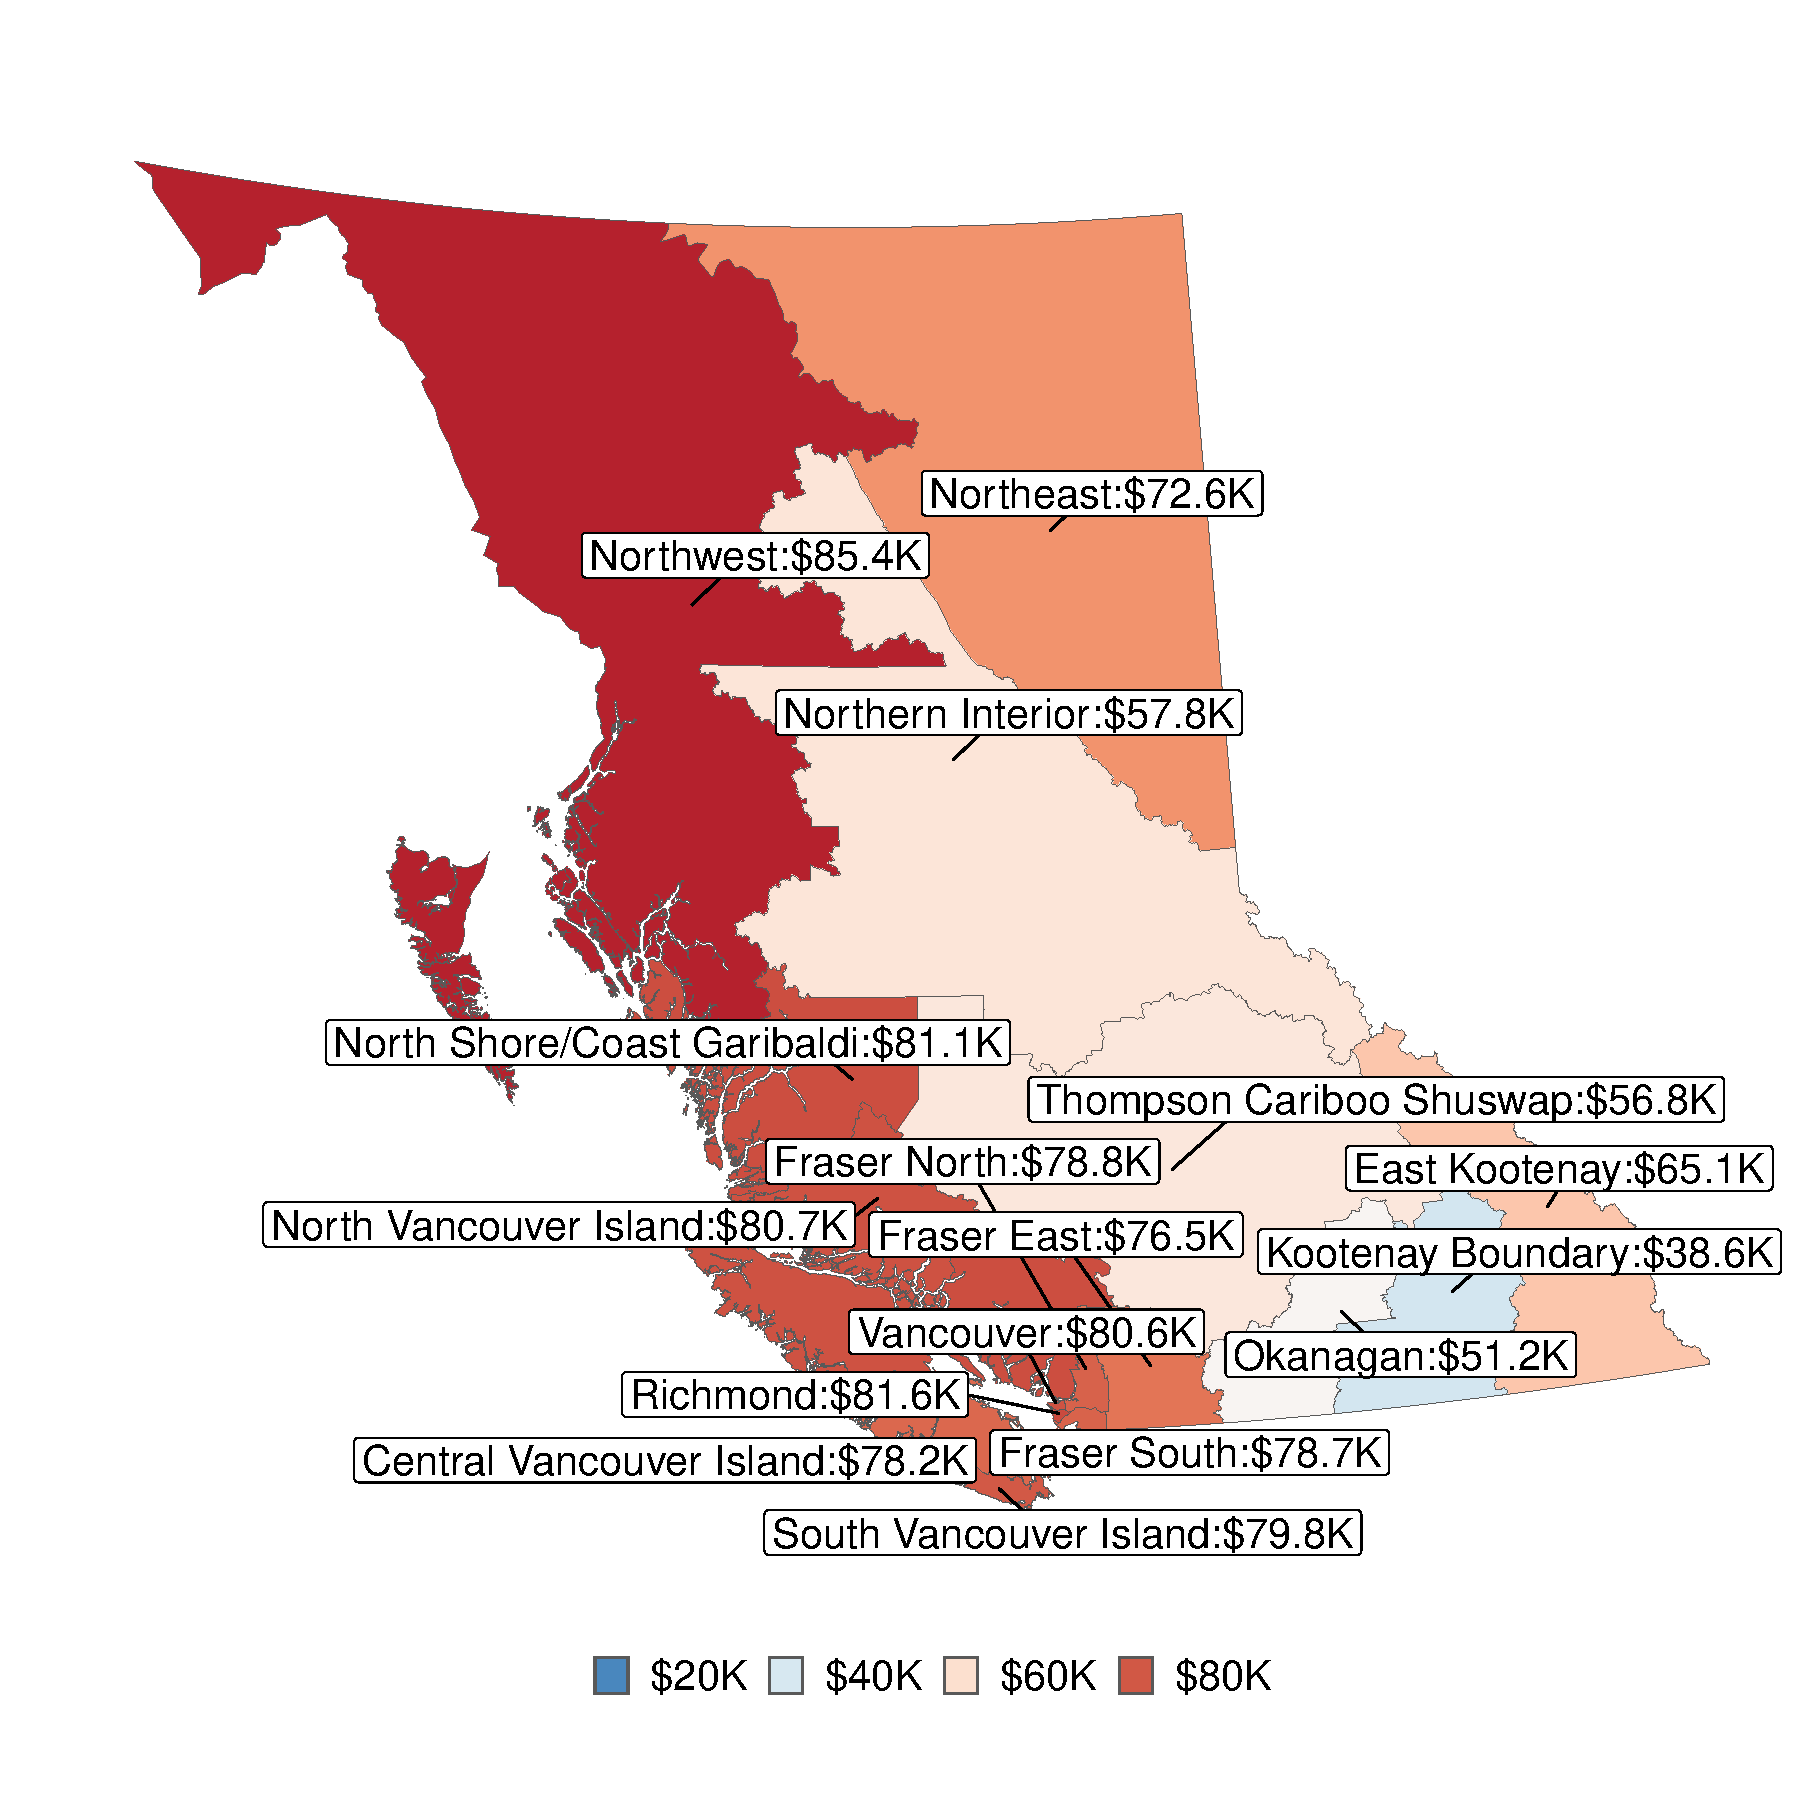
\includegraphics{index_files/figure-pdf/fig-ICER-1.pdf}

}

}

\subcaption{\label{fig-ICER-1}ICERs for the 100\% HEPA rebate program}
\end{minipage}%
%
\begin{minipage}[t]{0.50\linewidth}

{\centering 

\raisebox{-\height}{

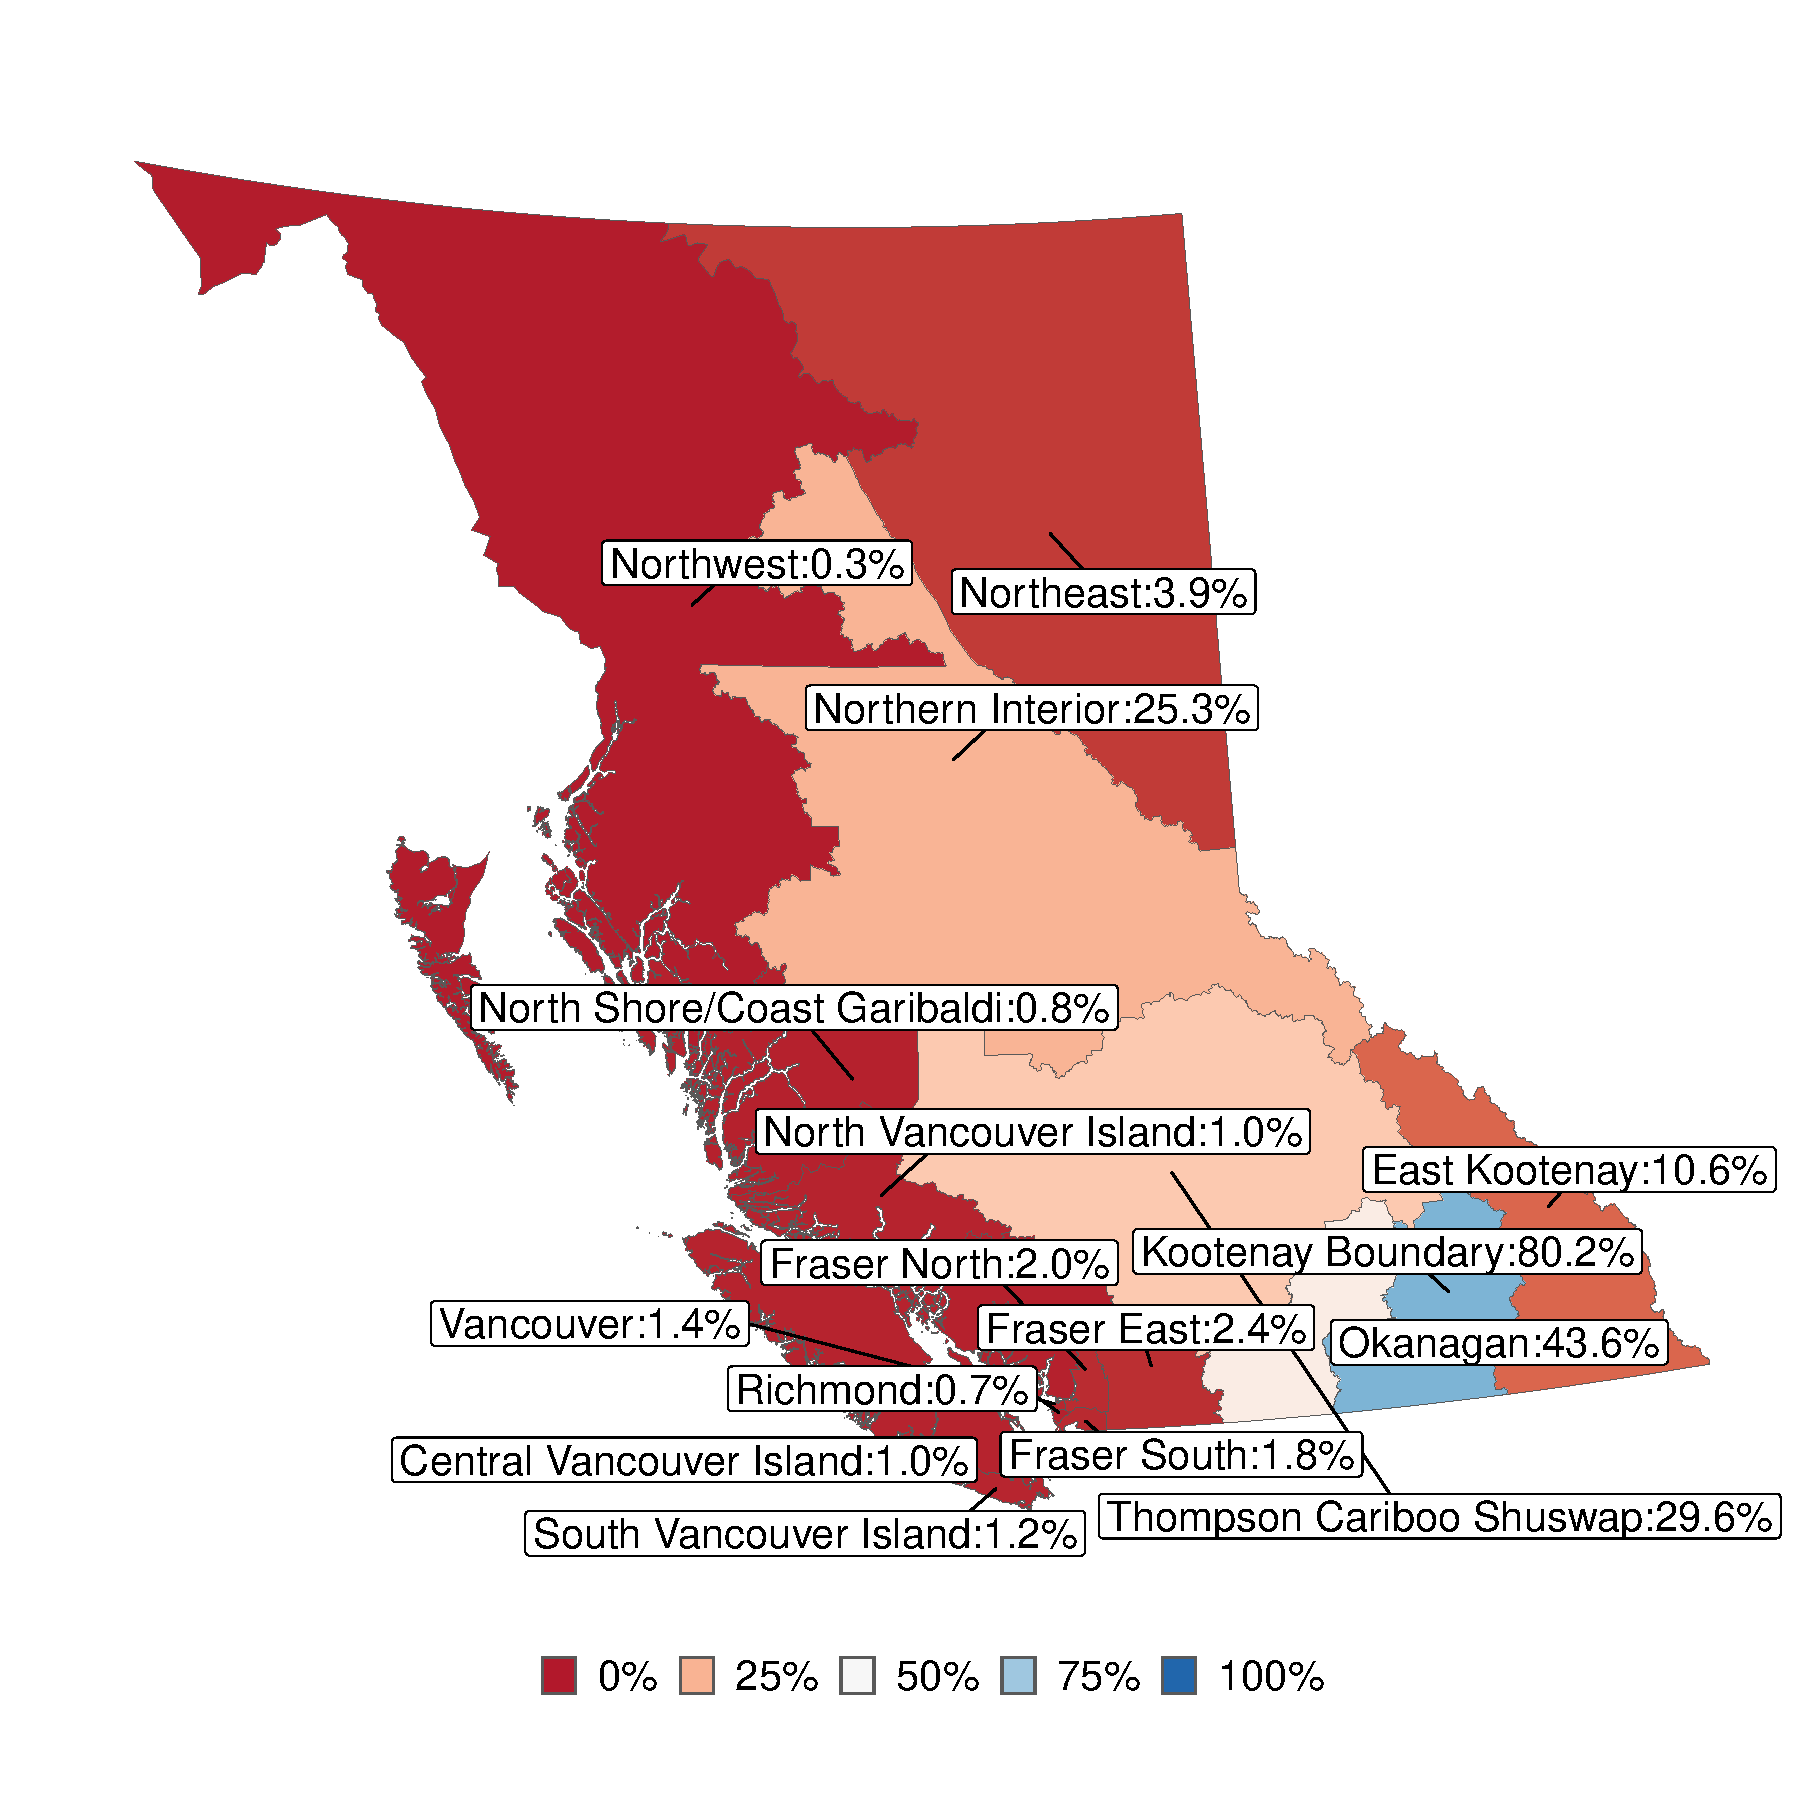
\includegraphics{index_files/figure-pdf/fig-ICER-2.pdf}

}

}

\subcaption{\label{fig-ICER-2}Cost-effectiveness probability at
WTP=\$50,000/QALY}
\end{minipage}%

\caption{\label{fig-ICER}Base-case results}

\end{figure}

Table~\ref{tbl-ICER} ranks HSDAs in BC in terms of HEPA rebate program
cost-effectiveness, in descending order based on ICER. ICERs ranged from
\$38,628/QALY in Kootenay Boundary to \$85,445/QALY in Northwest. Based
on model projections and prevalence of asthma in BC, a total of 4,536
severe exacerbations leading to systemic corticosteroids use, 531
emergency department visits, and 458 cases of hospitalizations could be
averted by continuous HEPA air filter use. Due to the larger populations
and higher prevalence of asthma, the highest number of severe
exacerbations averted (including systemic corticosteroids use, emergency
department visits, and hospitalizations) were in Fraser South (968),
Fraser North (649), Okanagan (611), and Vancouver (594).

Cost-effectiveness probabilities were highest in Kootenay Boundary
(80.2\%), Okanagan (43.6\%), and Thomson Cariboo Shuswap (29.6\%) HSDAs.
One-way sensitivity analysis (Appendix) showed that costs and QALYs were
most sensitive to the risk ratios of increased salbutamol dispensation
and hospitalization per 10 µg/m³ increase in PM\textsubscript{2.5},
utility of well-controlled and uncontrolled asthma, and the retail price
of air filter units.

\hypertarget{tbl-ICER}{}
\setlength{\LTpost}{0mm}
\begin{longtable}{lrrrrrrrr}
\caption{\label{tbl-ICER}ICERs for the portable HEPA air cleaner rebate program in BC }\tabularnewline

\toprule
 &  &  &  & \multicolumn{3}{c}{ΔExacerbation} &  &  \\ 
\cmidrule(lr){5-7}
HSDA & ΔCost & ΔQALY & ICER & SCS\textsuperscript{\textit{1}} & ED\textsuperscript{\textit{1}} & Hosp\textsuperscript{\textit{1}} & P\_CE\textsuperscript{\textit{2}} & NMB\textsuperscript{\textit{3}} \\ 
\midrule
Kootenay Boundary & $\text{\$}70.9$ & $0.0018$ & $\text{\$}38,628$ & $115$ & $14$ & $12$ & $80.2\%$ & $\text{\$}20.6$ \\ 
Okanagan & $\text{\$}77.1$ & $0.0015$ & $\text{\$}51,231$ & $501$ & $59$ & $51$ & $43.6\%$ & $-\text{\$}1.6$ \\ 
Thompson Cariboo Shuswap & $\text{\$}79.2$ & $0.0014$ & $\text{\$}56,806$ & $298$ & $35$ & $30$ & $29.6\%$ & $-\text{\$}9.7$ \\ 
Northern Interior & $\text{\$}79.5$ & $0.0014$ & $\text{\$}57,759$ & $170$ & $20$ & $17$ & $25.3\%$ & $-\text{\$}10.5$ \\ 
East Kootenay & $\text{\$}81.8$ & $0.0013$ & $\text{\$}65,103$ & $70$ & $8$ & $7$ & $10.6\%$ & $-\text{\$}18.8$ \\ 
Northeast & $\text{\$}83.7$ & $0.0011$ & $\text{\$}72,647$ & $53$ & $6$ & $5$ & $3.9\%$ & $-\text{\$}26.2$ \\ 
Fraser East & $\text{\$}84.6$ & $0.0011$ & $\text{\$}76,537$ & $357$ & $42$ & $36$ & $2.4\%$ & $-\text{\$}29.6$ \\ 
Central Vancouver Island & $\text{\$}84.9$ & $0.0011$ & $\text{\$}78,162$ & $275$ & $32$ & $28$ & $1.0\%$ & $-\text{\$}30.4$ \\ 
Fraser South & $\text{\$}85.0$ & $0.0011$ & $\text{\$}78,726$ & $795$ & $93$ & $80$ & $1.8\%$ & $-\text{\$}31.0$ \\ 
Fraser North & $\text{\$}85.1$ & $0.0011$ & $\text{\$}78,845$ & $533$ & $62$ & $54$ & $2.0\%$ & $-\text{\$}31.1$ \\ 
South Vancouver Island & $\text{\$}85.3$ & $0.0011$ & $\text{\$}79,838$ & $344$ & $40$ & $35$ & $1.2\%$ & $-\text{\$}31.8$ \\ 
Vancouver & $\text{\$}85.4$ & $0.0011$ & $\text{\$}80,556$ & $488$ & $57$ & $49$ & $1.4\%$ & $-\text{\$}32.4$ \\ 
North Vancouver Island & $\text{\$}85.4$ & $0.0011$ & $\text{\$}80,662$ & $119$ & $14$ & $12$ & $1.0\%$ & $-\text{\$}32.4$ \\ 
North Shore/Coast Garibaldi & $\text{\$}85.5$ & $0.0010$ & $\text{\$}81,115$ & $223$ & $26$ & $22$ & $0.8\%$ & $-\text{\$}33.0$ \\ 
Richmond & $\text{\$}85.6$ & $0.0010$ & $\text{\$}81,569$ & $135$ & $16$ & $14$ & $0.7\%$ & $-\text{\$}33.1$ \\ 
Northwest & $\text{\$}86.4$ & $0.0010$ & $\text{\$}85,445$ & $60$ & $7$ & $6$ & $0.3\%$ & $-\text{\$}35.9$ \\ 
\bottomrule
\end{longtable}
\begin{minipage}{\linewidth}
\textsuperscript{\textit{1}}SCS, ED, and Hosp denote excerbations requiring systemic corticosteroid therapy, emergency department vist, and hospitalization, respectively.\\
\textsuperscript{\textit{2}}P\_CE=Probability of Cost-Effectiveness based on probabilistic sensitivity analysis.\\
\textsuperscript{\textit{3}}NMB=Net Monetary Benefit\\
\end{minipage}

\hypertarget{scenario-analyses}{%
\subsection{Scenario Analyses}\label{scenario-analyses}}

Figure~\ref{fig-scenarios} shows results of scenario analyses. Our
results suggest that a \$100 rebate program would have been
cost-effective at a WTP threshold of \$50,000/QALY everywhere in the
province except for the Northwest HSDA, in which the ICER was
\$50,800/QALY.

The next two scenarios are based on operation of HEPA filters when the
outdoor PM\textsubscript{2.5} exceed a threshold concentration. We used
a threshold of 25 μg/m\textsuperscript{3} for PM\textsubscript{2.5},
based on the BC government 24-hour ambient air quality objective which
is used, along with other information to guide decisions on when to
issue an air quality advisory
\citep{ministryofenvironmentandclimatechangestrategy}.

Days with PM\textsubscript{2.5} concentrations above 25
μg/m\textsuperscript{3} were most common in August, followed by
September, July, October, and May. Our results suggest that a full
purchase rebate along with operation of air filters on days in which
outdoor PM\textsubscript{2.5} concentrations exceeded 25
μg/m\textsuperscript{3} would not have been cost-effective anywhere in
BC.

The last scenario considered a combination of a \$30 rebate and
operation of air filters on days in which PM\textsubscript{2.5}
concentrations exceeded 25 μg/m\textsuperscript{3}. Our results suggest
that the intervention would have been cost-effective in Kootenay
Boundary, Okanagan, Thompson Cariboo Shuswap, and Northern Interior.

\begin{figure}

\begin{minipage}[t]{0.33\linewidth}

{\centering 

\raisebox{-\height}{

\includegraphics{index_files/figure-pdf/fig-scenarios-1.pdf}

}

}

\subcaption{\label{fig-scenarios-1}Scenario 1, \$100 rebate}
\end{minipage}%
%
\begin{minipage}[t]{0.33\linewidth}

{\centering 

\raisebox{-\height}{

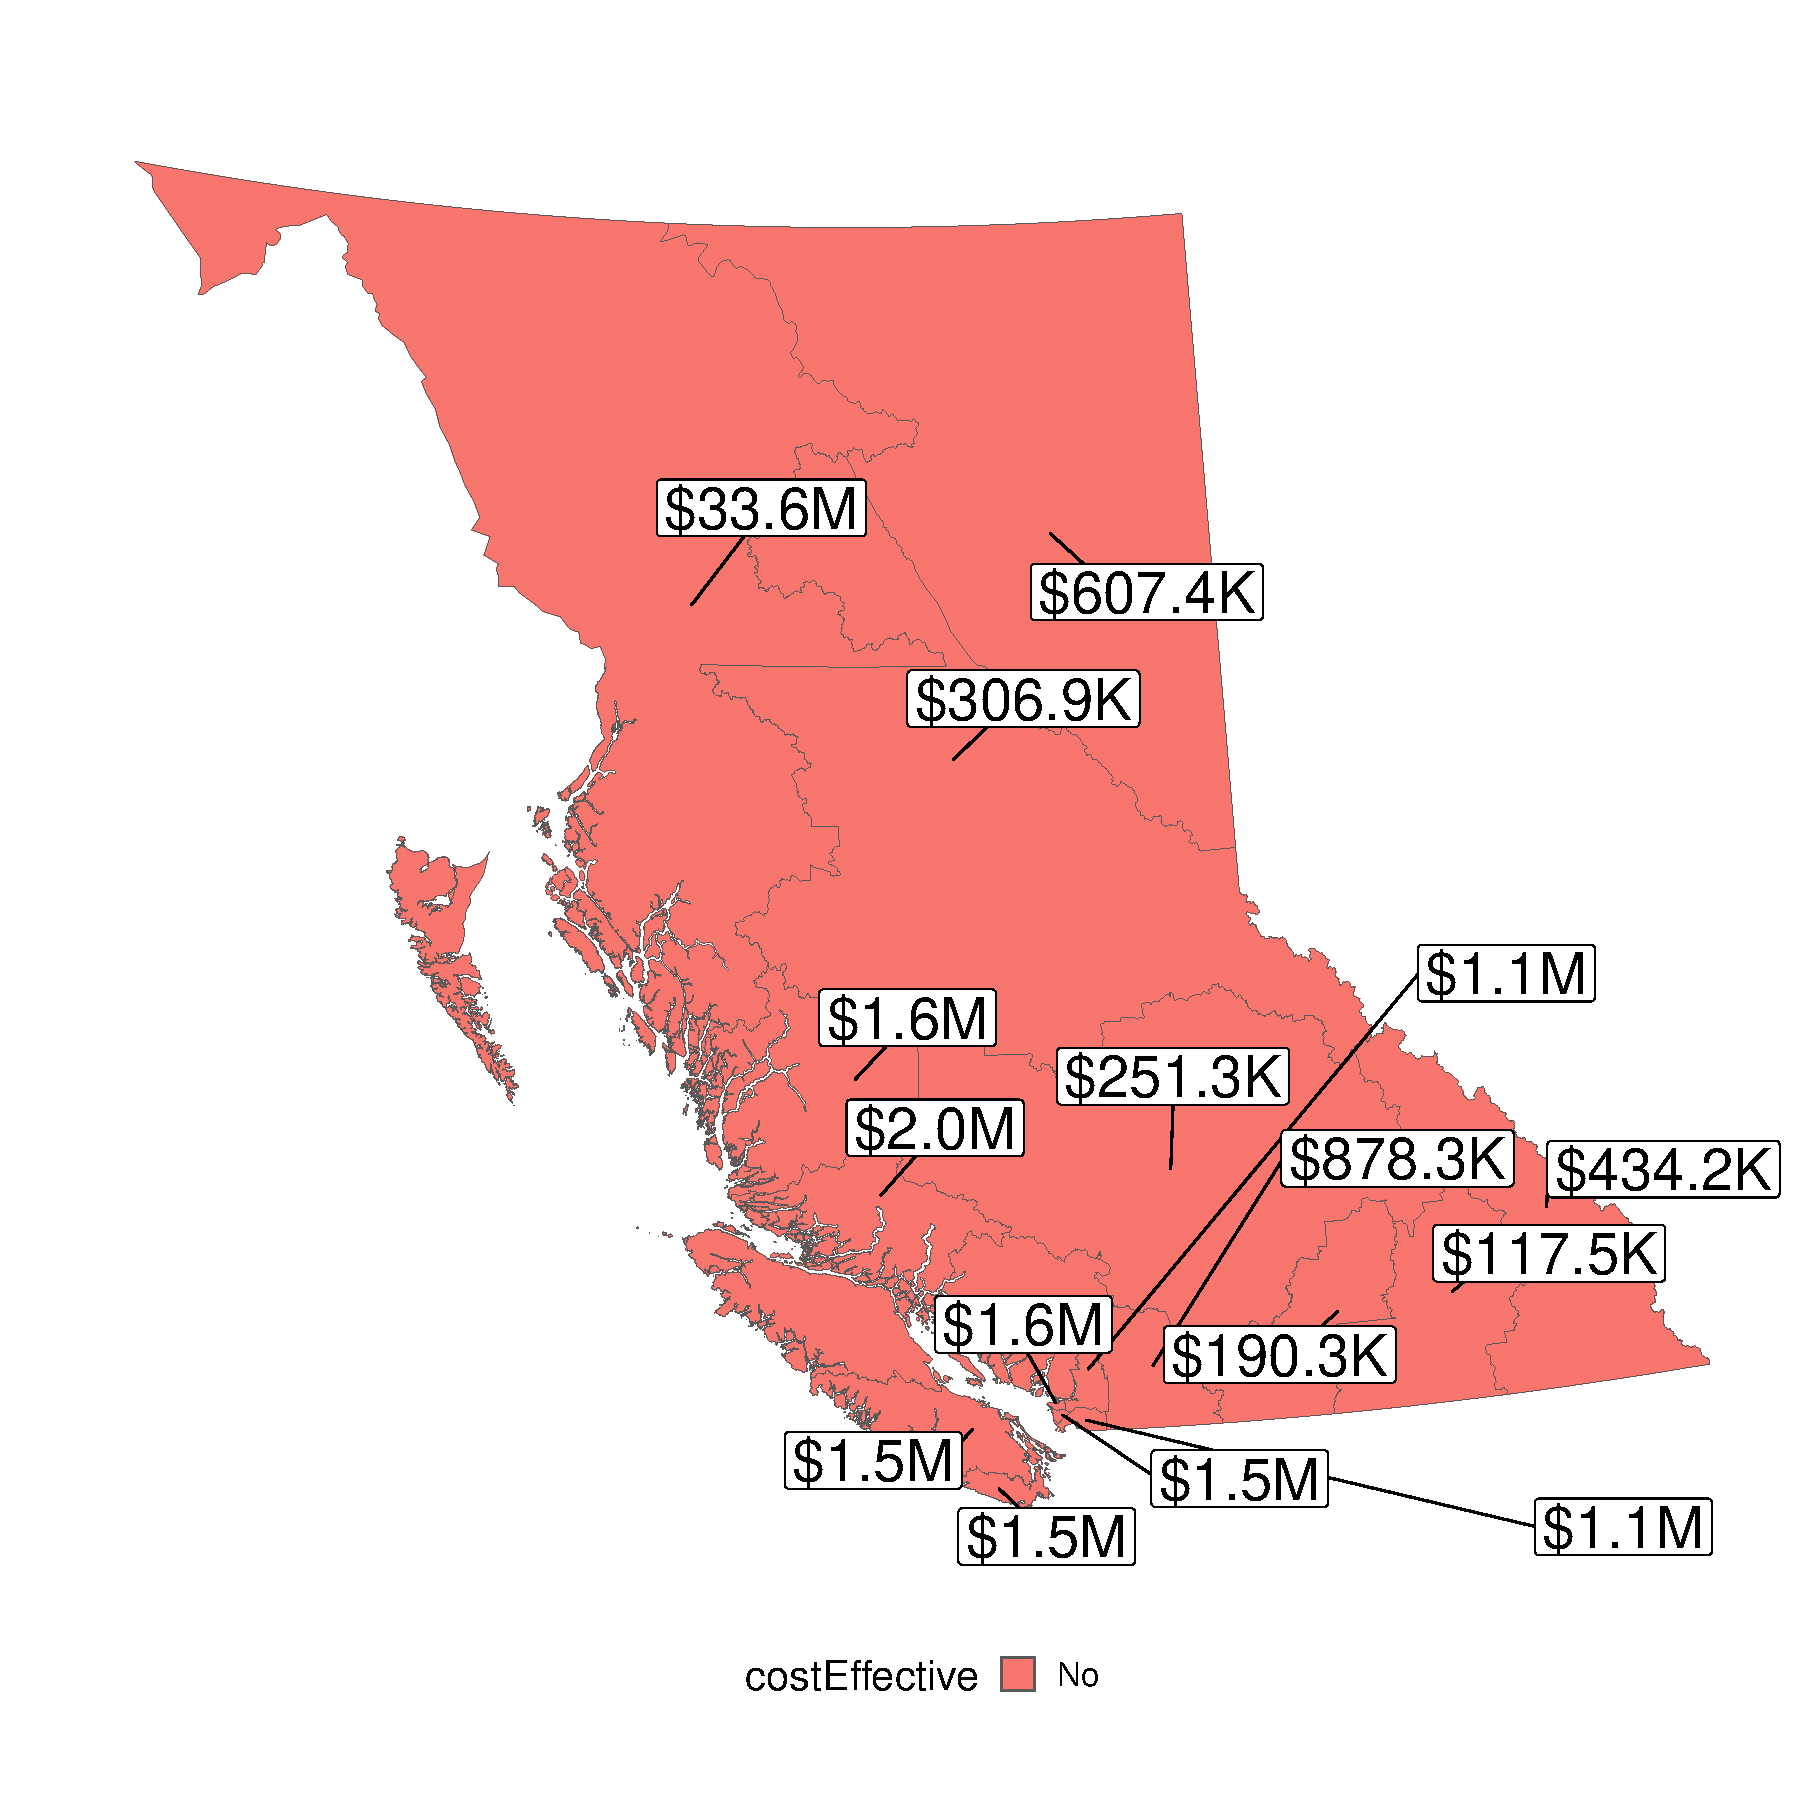
\includegraphics{index_files/figure-pdf/fig-scenarios-2.pdf}

}

}

\subcaption{\label{fig-scenarios-2}Scenario 2, Full rebate and air
filters on when PM2.5≥25μg/m3}
\end{minipage}%
%
\begin{minipage}[t]{0.33\linewidth}

{\centering 

\raisebox{-\height}{

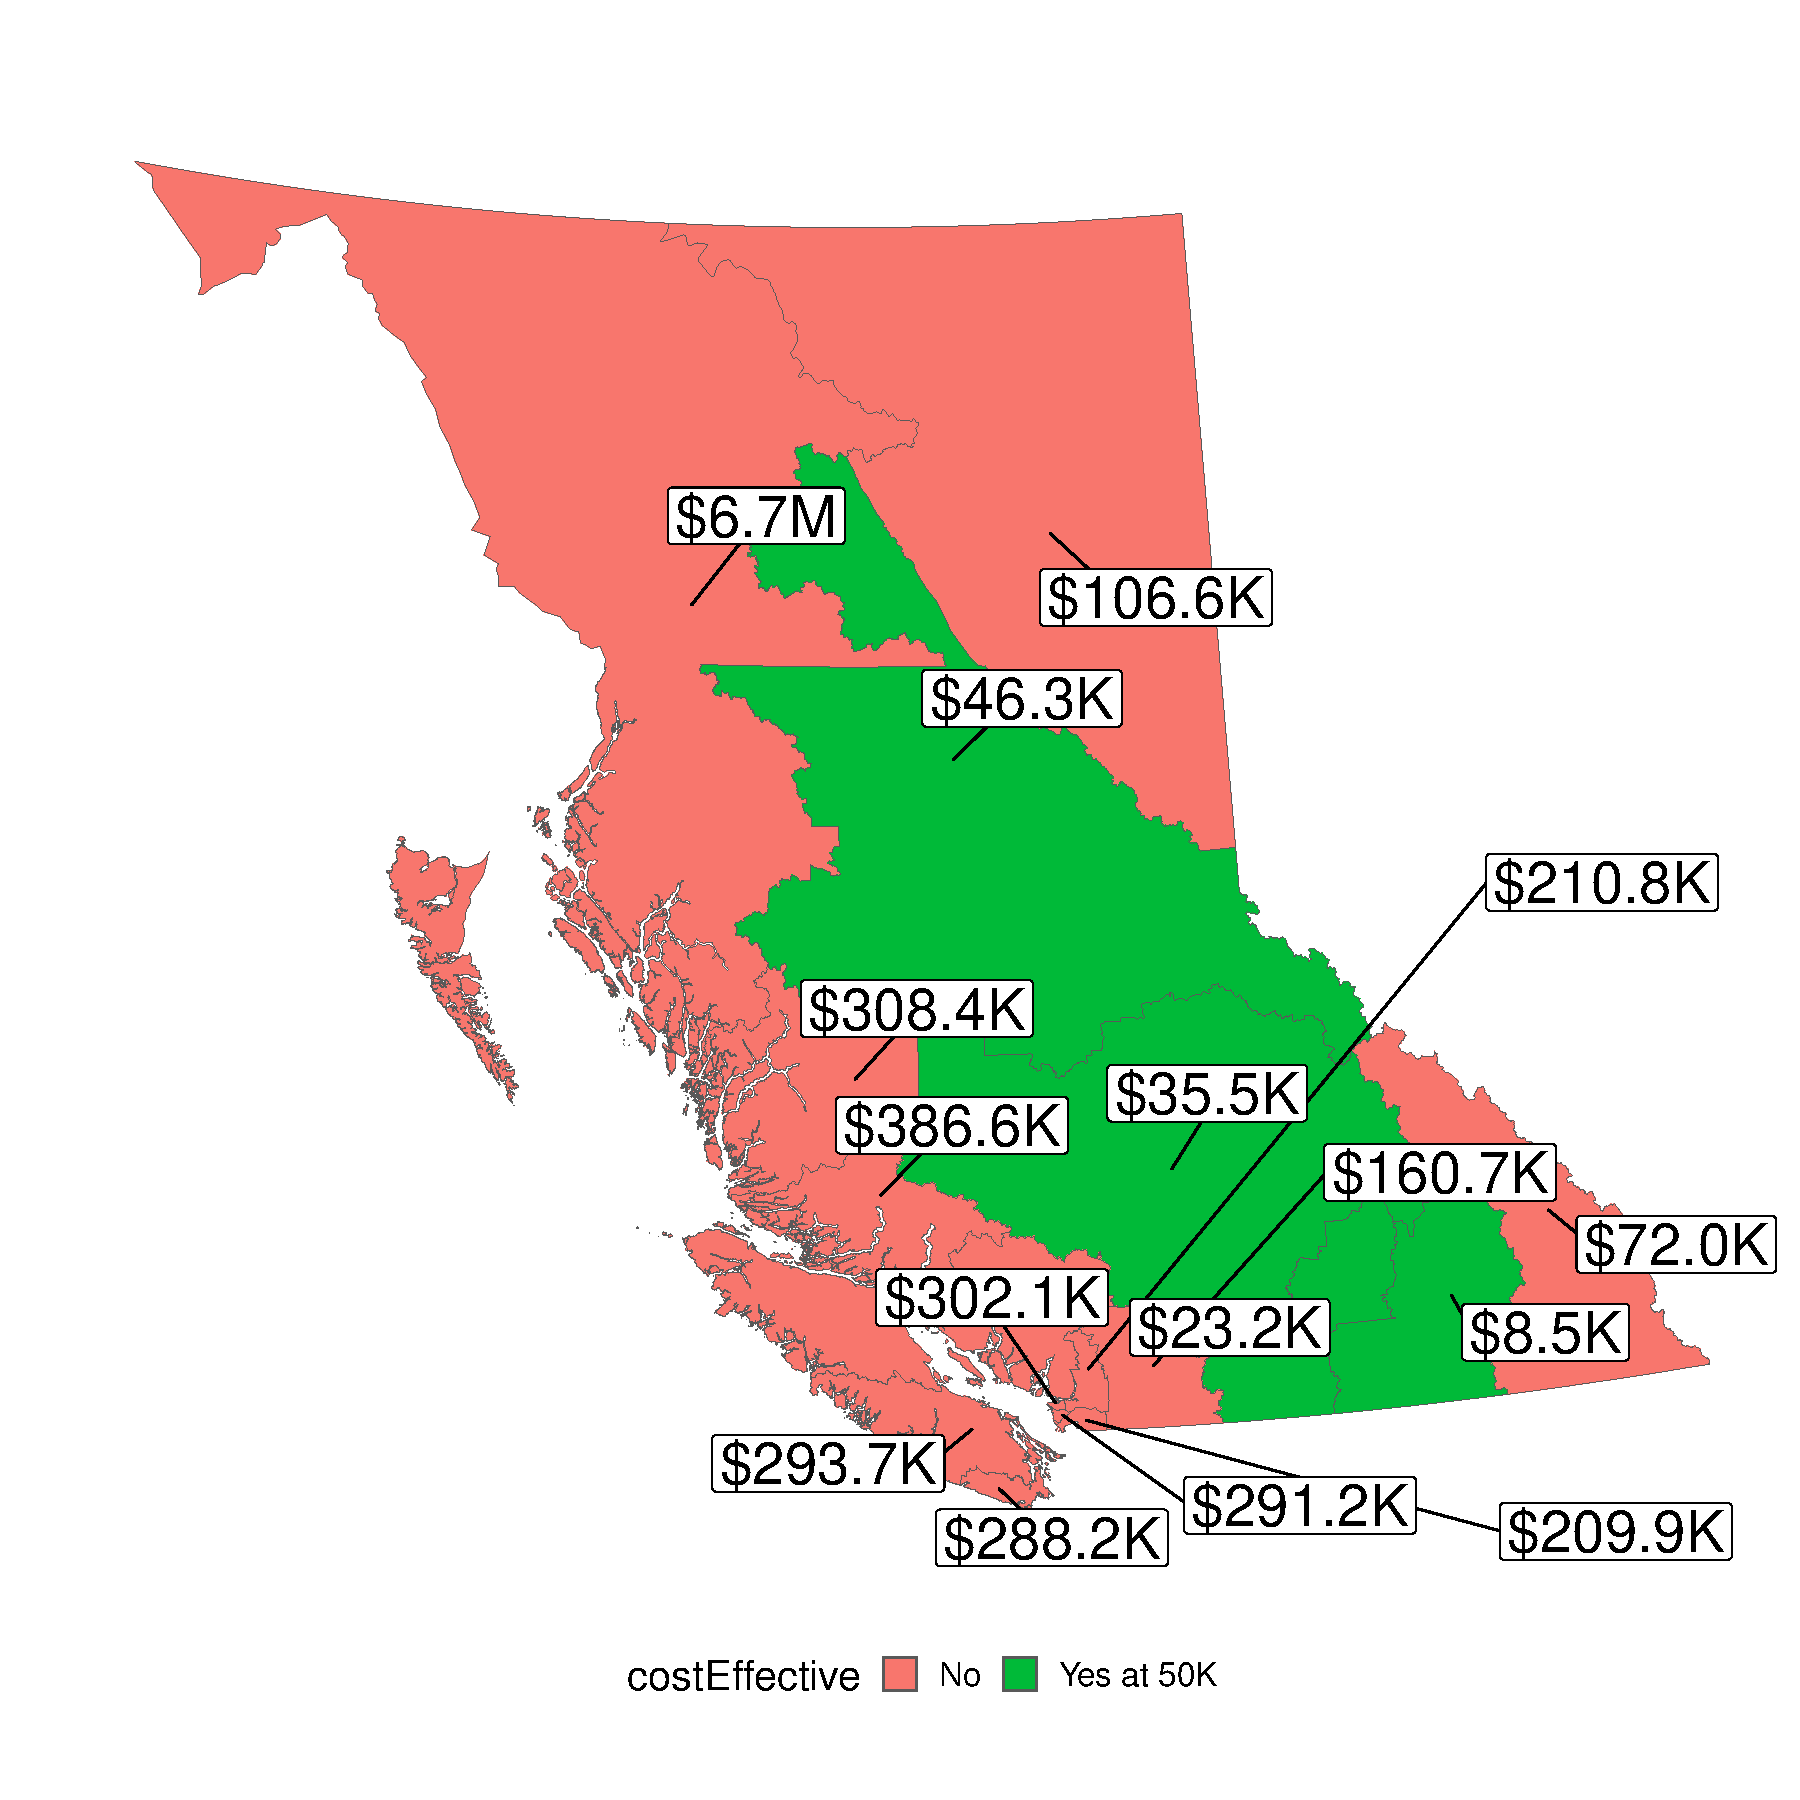
\includegraphics{index_files/figure-pdf/fig-scenarios-3.pdf}

}

}

\subcaption{\label{fig-scenarios-3}Scenario 3, \$30 rebate and air
filters on when PM2.5≥25μg/m3}
\end{minipage}%

\caption{\label{fig-scenarios}ICERs for HEPA Rebate Program - Different
Scenarios}

\end{figure}

\hypertarget{operation-costs}{%
\subsection{Operation Costs}\label{operation-costs}}

While a formal evaluation of the intervention from a societal
perspective is beyond the scope of this work, operation costs for
patients were calculated to provide additional context. In the base case
analysis when the air filter is operating continuously at its highest
setting, patients anywhere in BC can expect to pay an average of \$10
for 87.60 kWh of electricity and \$40 for HEPA filter replacements
annually, for a total of \$50 per year. In the threshold-based
scenarios, operation costs would be much lower (between \$0.03 to
\$1.91) and across different HSDAs as shown in the Appendix
Table~\ref{tbl-operationCost}.

\hypertarget{discussion}{%
\section{Discussion}\label{discussion}}

We found that across BC, offering a 100\% rebate on HEPA air filters was
cost-effective between 2018-2022 in Kootenay Boundary HSDA, which is the
most wildfire prone HSDA in the province. Our results suggest that a
\$100 rebate program was cost-effective in most of the province when air
filters were used continuously throughout the year. When air filters are
only operated on days in which PM\textsubscript{2.5} levels exceed 25
μg/m\textsuperscript{3}, a \$30 rebate program was also cost-effective
in wildfire-prone areas of the interior and northern interior BC. To the
best of our knowledge, this is the first cost-effectiveness analysis of
a government-sponsored HEPA air filter rebate program designed to
prevent wildfire smoke-related asthma exacerbations and improve asthma
control.

Particulate matter pollution is a major cause of health and economic
burden in Canada. In its 2022 report on the health of Canadians in a
changing climate, Health Canada classified fine particulate matter among
the three major outdoor pollutants which are collectively responsible
for 15,300 premature deaths in Canada annually, with an economic cost of
\$114 billion \citep{healthcanada2022}.

There are growing calls for governments to better protect health,
including by covering the cost of climate adaptation measures that
protect the public. For example, the BC Coroner's report on the 2021
heat dome in BC, which resulted in 619 deaths, recommended that the BC
government increase accessibility of air conditioners for use during
extreme events by allowing them to be provided as medical devices
through existing provincial programs \citep{thebccoronersservice2022}.
Heat events and smoke can occur together and the current public health
advice for the public is to create or access cool environments with
clean air. Our results suggest that a similar program should be
implemented for HEPA filter air cleaners to mitigate the impacts of
extreme wildfire events in HSDAs with recurrently high wildfire smoke
exposure.

We made several assumptions to develop our cost-effectiveness model.
Where possible, we opted for assumptions that would minimize the chance
of wrongly identifying the intervention as cost-effective. For instance,
we narrowly focused on the short-term health benefits of HEPA filters in
preventing acute asthma complications. However, chronic exposure to
wildfire smoke may also be associated with increased risk of asthma
incidence. Maintaining asthma control and preventing exacerbations is
likely associated with improved long-term respiratory outcomes, which
were not accounted for in our analysis. We only considered the benefits
of air filters in reducing exposure to wildfire-related
PM\textsubscript{2.5}. However, HEPA air filters reduce concentrations
of PM\textsubscript{2.5} from all sources, including traffic and
industry, indoor sources, allergens, bacteria, and respiratory viruses
such as flu and COVID-19. We also assumed that HEPA air filter units
would last only five years, regardless of how much they were in use,
while the HEPA filters had to be replaced every 9 months.

In our base case analysis, we assumed the air filter to be turned on
continuously for the 5-year time-horizon of the model, which is in line
with Health Canada's guideline that asserts there is no threshold of
exposure to PM\textsubscript{2.5} at which health effects may not
occur\citep{healthcanada2012}. Continuous operation of air filters also
ensures further benefits from reducing exposure to indoor sources of
PM\textsubscript{2.5}, allergens, and reduced transmission of
respiratory infections.

Our scenario analyses also showed that continuous operation of the HEPA
air filter is more beneficial than turning it on and off daily based on
the provincial 24-hour PM\textsubscript{2.5} ambient air quality
objective. It makes sense for the continuous operation to be the most
cost-effective choice from the government's perspective since there is
more benefit to reap with no additional cost as the government is only
paying for the upfront cost of a rebate.

Several limitations should be noted. First, the stochastic and
hard-to-predict nature of wildfire events prevented us from conducting
this analysis prospectively, as long-term prediction of wildfire events
in BC with adequate spatial and temporal resolution are not available.
Our retrospective results are still useful for future planning, as the
frequency and intensity of wildfires in BC is expected to grow, and
higher levels of exposure will make the intervention more
cost-effective.

Second, retrospective wildfire-related PM\textsubscript{2.5}
concentrations used in this study are based on the results of the
CanOSSEM model, and thus subject to limitations and uncertainties of
that model.

Third, within the observed PM\textsubscript{2.5} concentration range of
2.3 μg/m\textsuperscript{3} to 417.3 μg/m\textsuperscript{3}, we have
assumed a linear dose-response relationship for increased risk of change
in asthma control and asthma exacerbations leading to either SCS, ED
visit, or hospitalizations.

Lastly, due to a lack of data, we did not evaluate HEPA air filters in
subgroups of the population based on sex, age, ethnicity, or social
determinants of health, despite their established impact on the burden
of the disease\citep{chowdhury2021, schröder2015, karunanayake2020}.

\hypertarget{conclusion}{%
\section{Conclusion}\label{conclusion}}

Between 2018 and 2022, offering a 100\% rebate on portable HEPA air
filters was a cost-effective intervention to reduce short-term asthma
complications due to wildfire smoke in Kootenay Boundary but not in
other HSDAs in BC. Consumer rebates of up to \$100 (about two-thirds of
the cost of the air filter unit) were a cost-effective alternative in
most of the province, especially the interior and northern interior
parts of the province where wildfire exposure is higher.

\hypertarget{acknowledgments}{%
\section{Acknowledgments}\label{acknowledgments}}

We would like to acknowledge that most of the activities of this
research project were conducted on the traditional, ancestral, and
unceded territory of the Musqueam people.\\
We would like to thank our patient partners for sharing their feedback
and insights with us throughout this study. We are also thankful to our
knowledge user advisers Dr.~Michael Schwandt (Medical Health Officer,
Vancouver Coastal Health), Dr.~Silvina Mema (Medical Health Officer,
Interior Health), Paula Tait (Health \& Resource Development Technical
Adviser at Northern Health), and Jade Yehia (Environmental Health Policy
Lead at BC Ministry of Health). We would like to express our gratitude
Dr.~Mohsen Sadatsafavi (University of British Columbia) and Dr.~Zafar
Zafari (University of Maryland) for their help with health economics
methods. Lastly, we are very thankful to Dr.~Sarah Henderson and Naman
Paul (BC Centre for Disease Control) for sharing results of the CanOSSEM
model with us. This study was funded by Legacy for Airway Health.

\hypertarget{references}{%
\section{References}\label{references}}

\renewcommand{\bibsection}{}
\bibliography{references.bib}

\hypertarget{appendix-operation-costs}{%
\section{Appendix: Operation Costs}\label{appendix-operation-costs}}

\hypertarget{tbl-operationCost}{}
\begin{longtable}{lrr}
\caption{\label{tbl-operationCost}Average annual operation cost for patients under different scenarios }\tabularnewline

\toprule
HSDA & Base case, Scenario 1 & Scenarios 2 and 3 \\ 
\midrule
Central Vancouver Island & $\text{\$}50.00$ & $\text{\$}0.36$ \\ 
East Kootenay & $\text{\$}50.00$ & $\text{\$}1.61$ \\ 
Fraser East & $\text{\$}50.00$ & $\text{\$}0.70$ \\ 
Fraser North & $\text{\$}50.00$ & $\text{\$}0.61$ \\ 
Fraser South & $\text{\$}50.00$ & $\text{\$}0.55$ \\ 
Kootenay Boundary & $\text{\$}50.00$ & $\text{\$}1.91$ \\ 
North Shore/Coast Garibaldi & $\text{\$}50.00$ & $\text{\$}0.36$ \\ 
North Vancouver Island & $\text{\$}50.00$ & $\text{\$}0.25$ \\ 
Northeast & $\text{\$}50.00$ & $\text{\$}1.13$ \\ 
Northern Interior & $\text{\$}50.00$ & $\text{\$}1.20$ \\ 
Northwest & $\text{\$}50.00$ & $\text{\$}0.03$ \\ 
Okanagan & $\text{\$}50.00$ & $\text{\$}1.83$ \\ 
Richmond & $\text{\$}50.00$ & $\text{\$}0.36$ \\ 
South Vancouver Island & $\text{\$}50.00$ & $\text{\$}0.36$ \\ 
Thompson Cariboo Shuswap & $\text{\$}50.00$ & $\text{\$}1.66$ \\ 
Vancouver & $\text{\$}50.00$ & $\text{\$}0.36$ \\ 
\bottomrule
\end{longtable}

\hypertarget{appendix-deterministic-sensitivity-analysis}{%
\section{Appendix: Deterministic Sensitivity
Analysis}\label{appendix-deterministic-sensitivity-analysis}}

The following plots show the effect of changing input parameters on
overall ICER for each HSDA in each year.

\includegraphics{index_files/figure-pdf/unnamed-chunk-9-1.pdf}

\includegraphics{index_files/figure-pdf/unnamed-chunk-9-2.pdf}

\includegraphics{index_files/figure-pdf/unnamed-chunk-9-3.pdf}

\includegraphics{index_files/figure-pdf/unnamed-chunk-9-4.pdf}

\includegraphics{index_files/figure-pdf/unnamed-chunk-9-5.pdf}

\includegraphics{index_files/figure-pdf/unnamed-chunk-9-6.pdf}

\includegraphics{index_files/figure-pdf/unnamed-chunk-9-7.pdf}

\includegraphics{index_files/figure-pdf/unnamed-chunk-9-8.pdf}

\includegraphics{index_files/figure-pdf/unnamed-chunk-9-9.pdf}

\includegraphics{index_files/figure-pdf/unnamed-chunk-9-10.pdf}

\includegraphics{index_files/figure-pdf/unnamed-chunk-9-11.pdf}

\includegraphics{index_files/figure-pdf/unnamed-chunk-9-12.pdf}

\includegraphics{index_files/figure-pdf/unnamed-chunk-9-13.pdf}

\includegraphics{index_files/figure-pdf/unnamed-chunk-9-14.pdf}

\includegraphics{index_files/figure-pdf/unnamed-chunk-9-15.pdf}

\includegraphics{index_files/figure-pdf/unnamed-chunk-9-16.pdf}

\includegraphics{index_files/figure-pdf/unnamed-chunk-9-17.pdf}

\includegraphics{index_files/figure-pdf/unnamed-chunk-9-18.pdf}

\includegraphics{index_files/figure-pdf/unnamed-chunk-9-19.pdf}

\includegraphics{index_files/figure-pdf/unnamed-chunk-9-20.pdf}

\includegraphics{index_files/figure-pdf/unnamed-chunk-9-21.pdf}

\includegraphics{index_files/figure-pdf/unnamed-chunk-9-22.pdf}

\includegraphics{index_files/figure-pdf/unnamed-chunk-9-23.pdf}

\includegraphics{index_files/figure-pdf/unnamed-chunk-9-24.pdf}

\includegraphics{index_files/figure-pdf/unnamed-chunk-9-25.pdf}

\includegraphics{index_files/figure-pdf/unnamed-chunk-9-26.pdf}

\includegraphics{index_files/figure-pdf/unnamed-chunk-9-27.pdf}

\includegraphics{index_files/figure-pdf/unnamed-chunk-9-28.pdf}

\includegraphics{index_files/figure-pdf/unnamed-chunk-9-29.pdf}

\includegraphics{index_files/figure-pdf/unnamed-chunk-9-30.pdf}

\includegraphics{index_files/figure-pdf/unnamed-chunk-9-31.pdf}

\includegraphics{index_files/figure-pdf/unnamed-chunk-9-32.pdf}




\end{document}
